% This example is meant to be compiled with lualatex or xelatex
% The theme itself also supports pdflatex
\PassOptionsToPackage{unicode}{hyperref}
\documentclass[aspectratio=1610, 12pt, xcolor=dvipsnames]{beamer}

% Warning, if another latex run is needed
% \usepackage[aux]{rerunfilecheck}

% just list chapters and sections in the toc, not subsections or smaller
\setcounter{tocdepth}{1}

%------------------------------------------------------------------------------
%------------------------------ Fonts, Unicode, Language ----------------------
%------------------------------------------------------------------------------
\usepackage{fontspec}
\defaultfontfeatures{Ligatures=TeX}  % -- becomes en-dash etc.

% german language
\usepackage{polyglossia}
\setdefaultlanguage{german}

% for english abstract and english titles in the toc
\setotherlanguages{english}

% intelligent quotation marks, language and nesting sensitive
\usepackage[autostyle]{csquotes}

% microtypographical features, makes the text look nicer on the small scale
\usepackage{microtype}

% colors and stuff
\usepackage{xcolor}
\usepackage[most]{tcolorbox}
% Here was colback=SpringGreen before but it is not finding the xcolor package
\tcbset{on line,
        boxsep=4pt, left=0pt,right=0pt,top=0pt,bottom=0pt,
        colframe=white,colback=green,
        highlight math style={enhanced}
        }
\newtcolorbox{mybox}[3][]
{
  colframe = #2!25,
  colback = #2!20,
  coltitle = #2!20!black,
  title = {#3},
  #1
}
%\colorlet{Green!40}
%------------------------------------------------------------------------------
%------------------------ Math Packages and settings --------------------------
%------------------------------------------------------------------------------

\usepackage{amsmath}
\usepackage{amssymb}
\usepackage{mathtools}
\usepackage{bbold}

% Enable Unicode-Math and follow the ISO-Standards for typesetting math
\usepackage[
  math-style=ISO,
  bold-style=ISO,
  sans-style=italic,
  nabla=upright,
  partial=upright,
]{unicode-math}
\setmathfont{Latin Modern Math}

% nice, small fracs for the text with \sfrac{}{}
\usepackage{xfrac}


%------------------------------------------------------------------------------
%---------------------------- Numbers and Units -------------------------------
%------------------------------------------------------------------------------

\usepackage[
  locale=DE,
  separate-uncertainty=true,
  per-mode=symbol-or-fraction,
]{siunitx}
\sisetup{math-micro=\text{µ},text-micro=µ}
% \sisetup{tophrase={{ to }}}
%------------------------------------------------------------------------------
%-------------------------------- tables  -------------------------------------
%------------------------------------------------------------------------------

\usepackage{booktabs}       % \toprule, \midrule, \bottomrule, etc

%------------------------------------------------------------------------------
%-------------------------------- graphics -------------------------------------
%------------------------------------------------------------------------------

\usepackage{graphicx}
%\usepackage{rotating}
\usepackage{grffile}
\usepackage{tikz}
\usepackage{circuitikz}
\usepackage{tikz-feynman}
\usepackage{subcaption}

% allow figures to be placed in the running text by default:
\usepackage{scrhack}
\usepackage{float}
\floatplacement{figure}{htbp}
\floatplacement{table}{htbp}

% keep figures and tables in the section
\usepackage[section, below]{placeins}

% smileys
\usepackage{MnSymbol,wasysym}

%------------------------------------------------------------------------------
%---------------------- customize list environments ---------------------------
%------------------------------------------------------------------------------

\usepackage{enumitem}
\usepackage{listings}
\usepackage{hepunits}

\usepackage{pdfpages}
%------------------------------------------------------------------------------
%------------------------------ Bibliographie ---------------------------------
%------------------------------------------------------------------------------

\setbeamertemplate{itemize/enumerate body begin}{\tiny}
\setbeamertemplate{itemize/enumerate subbody begin}{\tiny}
\setbeamertemplate{itemize/enumerate subsubbody begin}{\tiny}
\usepackage{moresize}

\usepackage[
  backend=biber,   % use modern biber backend
  autolang=hyphen, % load hyphenation rules for if language of bibentry is not
                   % german, has to be loaded with \setotherlanguages
                   % in the references.bib use langid={en} for english sources
]{biblatex}
\addbibresource{references.bib}  % the bib file to use
\DefineBibliographyStrings{german}{andothers = {{et\,al\adddot}}}  % replace u.a. with et al.


% Load packages you need here
% \usepackage{polyglossia}
% \setmainlanguage{german}

\usepackage{csquotes}


% \usepackage{amsmath}
% \usepackage{amssymb}
% \usepackage{mathtools}

\usepackage{hyperref}
\usepackage{bookmark}

% load the theme after all packages

\usetheme[
  showtotalframes, % show total number of frames in the footline
]{tudo}

% Put settings here, like
\unimathsetup{
  math-style=ISO,
  bold-style=ISO,
  nabla=upright,
  partial=upright,
  mathrm=sym,
}

% \setbeamertemplate{itemize item}{\scriptsize$\blacktriangleright$}
% \setbeamertemplate{itemize subitem}{\scriptsize$\blacktriangleright$}

%Titel:
\title{SciFi reconstruction and alignment}
%Autor
\author[N.Breer]{\textbf{Nils Breer} + SciFi alignment + calibration team}
%Lehrstuhl/Fakultät
\institute{SciFi general at 108th LHCb week - 5th june 2023}
%Titelgrafik muss ich einfueren!!!
%\titlegraphic{\includegraphics[width=0.3\textwidth]{content/Bilder/interferenz.jpg}}
% \date{16.03.2023}

\begin{document}
\maketitle

\begin{frame}\frametitle{Reconstruction and alignment overview}
  \begin{columns}
    \begin{column}[c]{0.66\textwidth}
      \begin{itemize}
        \item $\bullet$\, SciFi simulation and reconstruction
        \begin{itemize}
          \item $\bullet$\, Weekly group meetings: Monday, 13:00h
          \item $\bullet$\, Mailing list: lhcb-upgrade-ft-software
          \item $\bullet$\, \href{https://twiki.cern.ch/twiki/bin/view/LHCb/SciFiSimulation}{Twiki}
        \end{itemize}
        \item $\bullet$\, Updates since \href{https://indico.cern.ch/event/1253790/}{last LHCb week}
        \begin{itemize}
          \item $\bullet$\, Alignment:
          \begin{itemize}
            \item $\bullet$\, published Alignment v10
            \item $\bullet$\, new and improved photogrammetry taken
            \item $\bullet$\, readout map improved
            \item $\bullet$\,
          \end{itemize}
        \end{itemize}
        % \item $\bullet$\, gutes bild in lhcb week 106 von sophie
      \end{itemize}
    \end{column}
    \begin{column}[c]{0.33\textwidth}
      \begin{itemize}
        \item \scriptsize \textbf{People working with SciFi}
        \item \textbf{align and calibration}
        \item $\bullet$\, Blake Leverington
        \item $\bullet$\, Fred Blanc
        \item $\bullet$\, Izaac Sanderswood
        \item $\bullet$\, Maria Vieites Diaz
        \item $\bullet$\, Zehua Xu
        \item $\bullet$\, Jessy Daniel
        \item $\bullet$\, Louis Henry
        \item $\bullet$\, Emmy Gabriel
        \item $\bullet$\, Sophie Hollitt
        \item $\bullet$\, Biljana Mitreska
        \item $\bullet$\, Miguel Ruiz Diaz
        \item $\bullet$\, Giulia Tuci
        \item \textbf{People from different projects}
        \item $\bullet$\, Laurent Dufour
        \item \textbf{SciFi in general, RTA alignment and reconstruction helped a lot during commissioning}
      \end{itemize}
      % \normalsize
    \end{column}
  \end{columns}
\end{frame}

\begin{frame}\frametitle{Overview of the topics}
\begin{figure}
  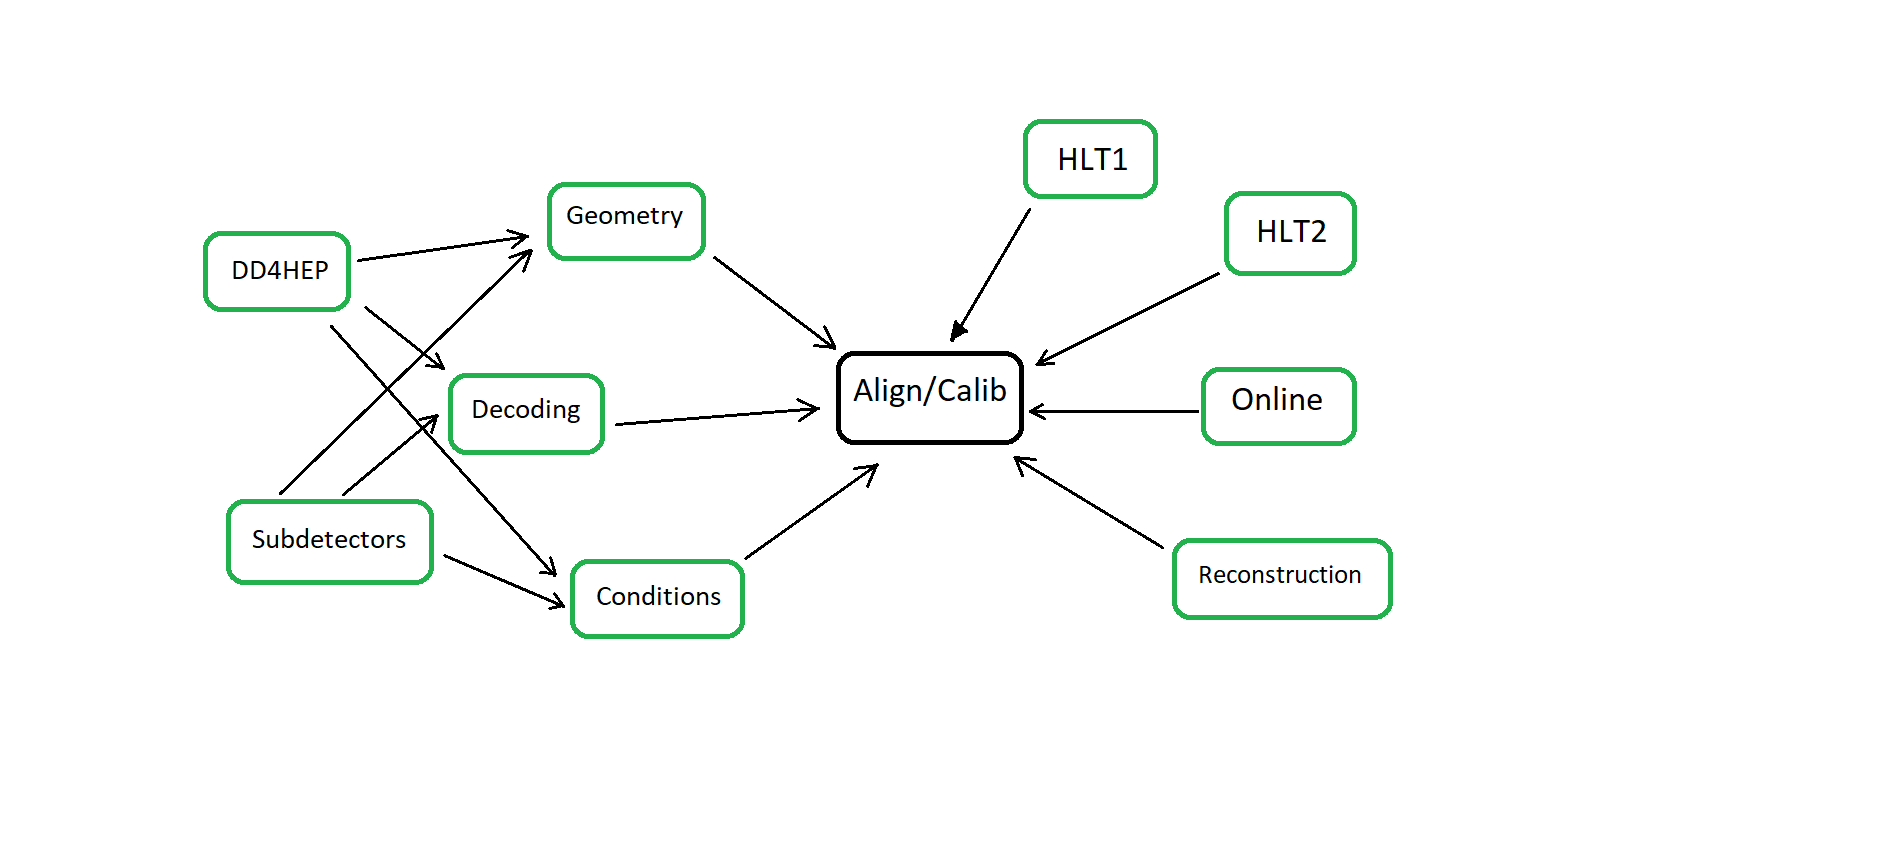
\includegraphics[width=0.9\textwidth]{plots/align_reco_overview.png}
\end{figure}
\end{frame}

\begin{frame}\frametitle{Readoup Map adaptations}
  \begin{columns}
    \begin{column}[c]{0.48\textwidth}
      \begin{itemize}
        \item Readout map \to Cabling Map
        \item automatic fetching of deactivated links
        \item \to deactivate links without changing readout map!
      \end{itemize}
    \end{column}
    \begin{column}[c]{0.48\textwidth}
      \begin{itemize}
        \item 2022: no active link map \to  empty events
        \item \href{https://gitlab.cern.ch/lhcb/LHCb/-/merge_requests/4129}{LHCb!4129} improved flexibility
        \item 2023: allows to ignore dynamic link deactivation if no active link found
      \end{itemize}
    \end{column}
  \end{columns}
\end{frame}

\begin{frame}\frametitle{Survey and Photogrammetry}
  \begin{columns}
    \begin{column}[c]{0.48\textwidth}
      \begin{figure}
        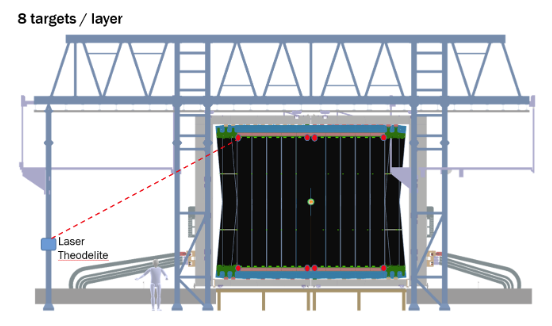
\includegraphics[width=0.9\textwidth]{plots/survey_photo.png}
      \end{figure}
    \end{column}
    \begin{column}[c]{0.48\textwidth}
      \begin{itemize}
        \item $\bullet$\, photogrammetry taken: feb 20th - march 9th
        \item $\bullet$\, 4 measurement points per C-frame at corners
        \item $\bullet$\, target: keep inner modules as close to nominal as possible, outer edges can move as needed
        \item $\bullet$\, summary: 450 microns in z, most frames within 200 microns from nominal
        \item $\bullet$\, 400 microns in x, 1.5 mm in y
        \item $\bullet$\, on average 400 - 600 microns in y, 50 - 200 microns in the center
      \end{itemize}
    \end{column}
  \end{columns}
\end{frame}

\begin{frame}\frametitle{Photogrammetry}
  \begin{columns}
    \begin{column}[c]{0.48\textwidth}
      \begin{figure}
        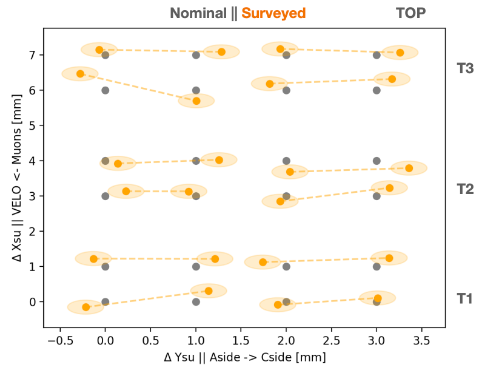
\includegraphics[width=0.5\textwidth]{plots/survey_top.png}
        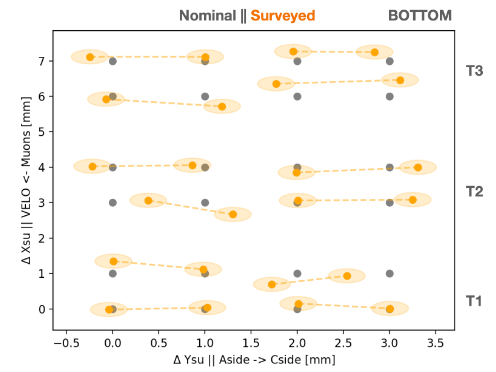
\includegraphics[width=0.5\textwidth]{plots/survey_bottom.png}
      \end{figure}
    \end{column}
    \begin{column}[c]{0.48\textwidth}
      \begin{itemize}
        \item $\bullet$\, top/bottom view of the respective edges $\pm 2.5m$ above/below beam pipe
        \item $\bullet$\, 200 $\mu m$ survey uncertainty
        \item $\bullet$\, A-side \to +x, C-side \to -x
        \item $\bullet$\, T1, T2: outer layers surveyed \to L0 and L3
      \end{itemize}
    \end{column}
  \end{columns}
\end{frame}

\begin{frame}\frametitle{Survey and Photogrammetry}
  \begin{columns}
    \begin{column}[c]{0.48\textwidth}
      \begin{figure}
        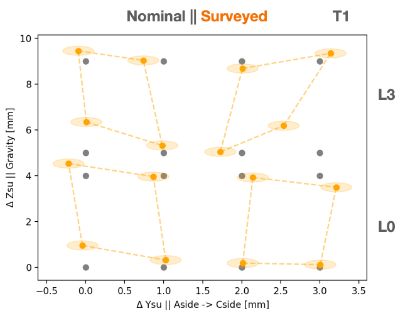
\includegraphics[width=0.5\textwidth]{plots/survey_T1.png}
        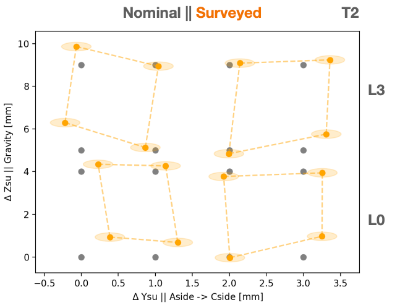
\includegraphics[width=0.5\textwidth]{plots/survey_T2.png}
      \end{figure}
    \end{column}
    \begin{column}[c]{0.48\textwidth}
      \begin{itemize}
        \item $\bullet$\, T3: L0 and L2 surveyed (L3 targets in RICH volume)
        \item $\bullet$\, T3L2 measured between L1 and L2 with smaller targets
        \item $\bullet$\, possible movement during measurement
      \end{itemize}
      \begin{figure}
        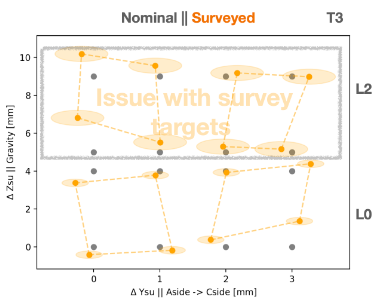
\includegraphics[width=0.5\textwidth]{plots/survey_T3.png}
      \end{figure}
    \end{column}
  \end{columns}
\end{frame}

\begin{frame}\frametitle{VELO drift situation}
  \begin{columns}
    \begin{column}[c]{0.48\textwidth}
      \begin{figure}
        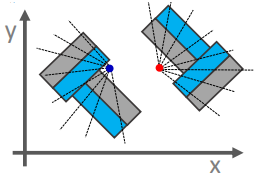
\includegraphics[width=0.5\textwidth]{plots/velo_axes.png}
        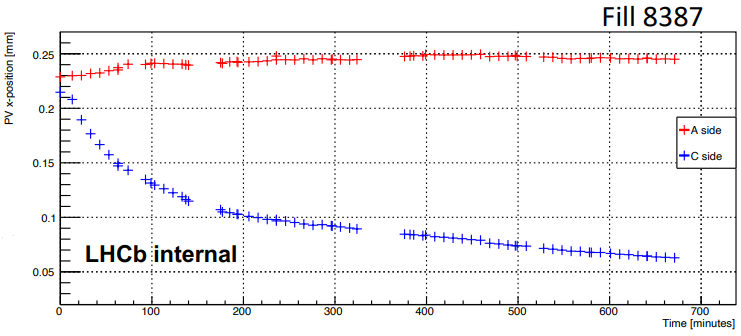
\includegraphics[width=0.5\textwidth]{plots/c_side_drift_freiss.png}
      \end{figure}
    \end{column}
    \begin{column}[c]{0.48\textwidth}
      \begin{itemize}
        \item $\bullet$\, The situation:
        \item $\bullet$\, Monitoring, alignment and material scan are consistent
        \item $\bullet$\, During closing, C-side starts rotating around y with pivot point at around 850 mm
        \item $\bullet$\, \to upstream region lacks behind
        \item $\bullet$\, complications:
        \begin{itemize}
          \item $\bullet$\, start of drift unpredictable
          \item $\bullet$\, drift amount differs over time
        \end{itemize}
      \end{itemize}
    \end{column}
  \end{columns}
\end{frame}

\begin{frame}\frametitle{VELO drift impact for SciFi alignment}
  \begin{columns}
    \begin{column}[c]{0.48\textwidth}
      \begin{itemize}
        \item $\bullet$\, Goal: estimate impact of VELO movement on reconstructed mass
        \item $\bullet$\, DoFs: Tx, Rz long modules aligned, GoodLongTracks
        \item $\bullet$\, data set: $\symup{B}_0 \to D^{*}\pi$ and $\symup{D}_0 \to \symup{K}\pi$
        % \item $\bullet$\,
      \end{itemize}
    \end{column}
    \begin{column}[c]{0.48\textwidth}
      \begin{figure}
        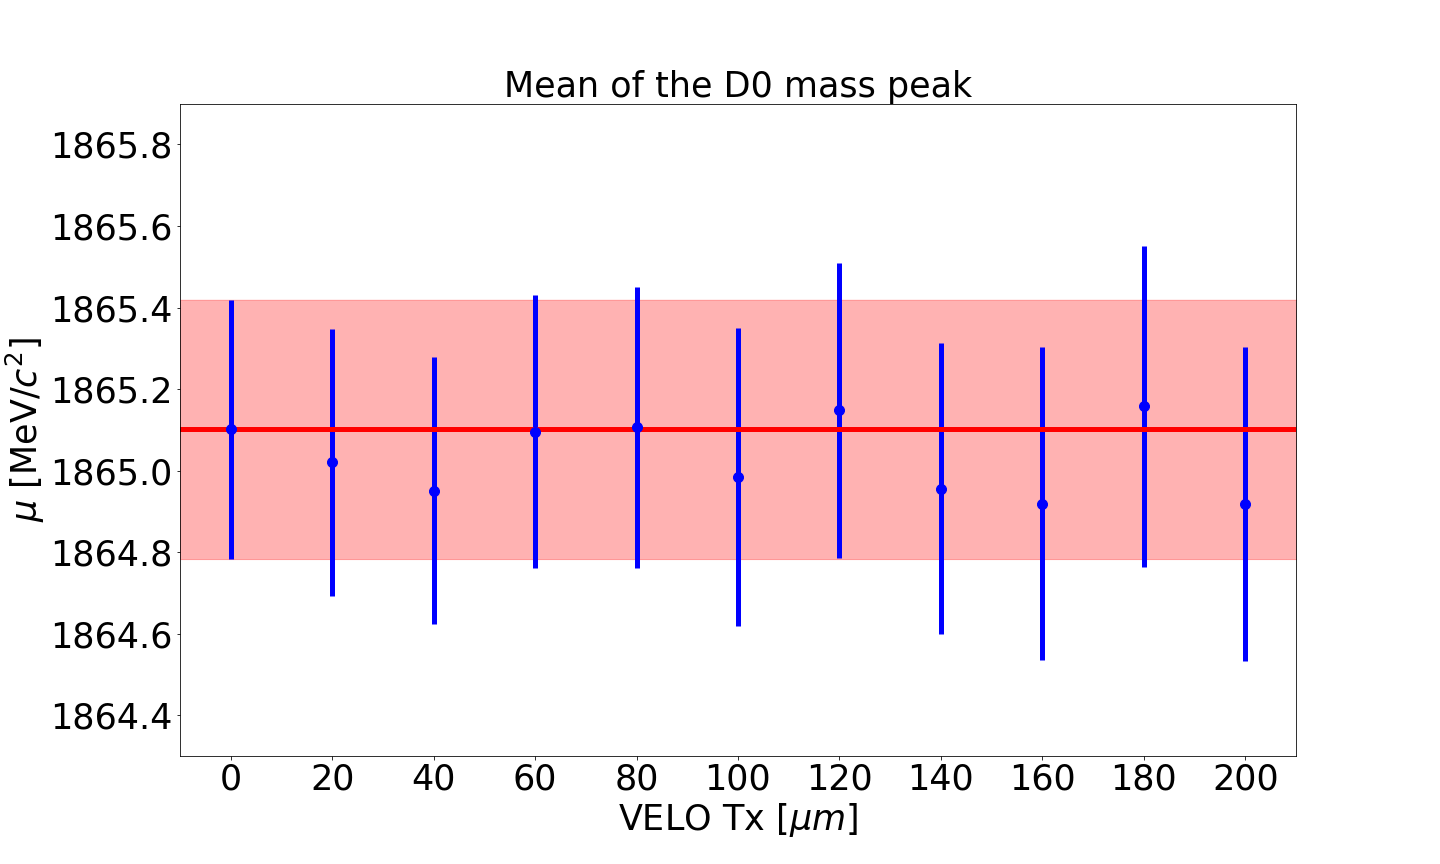
\includegraphics[width=0.5\textwidth]{reading_material/current_stuff/velo_drift_plots/plots/D0_massvalue_smallVPTx.png}
        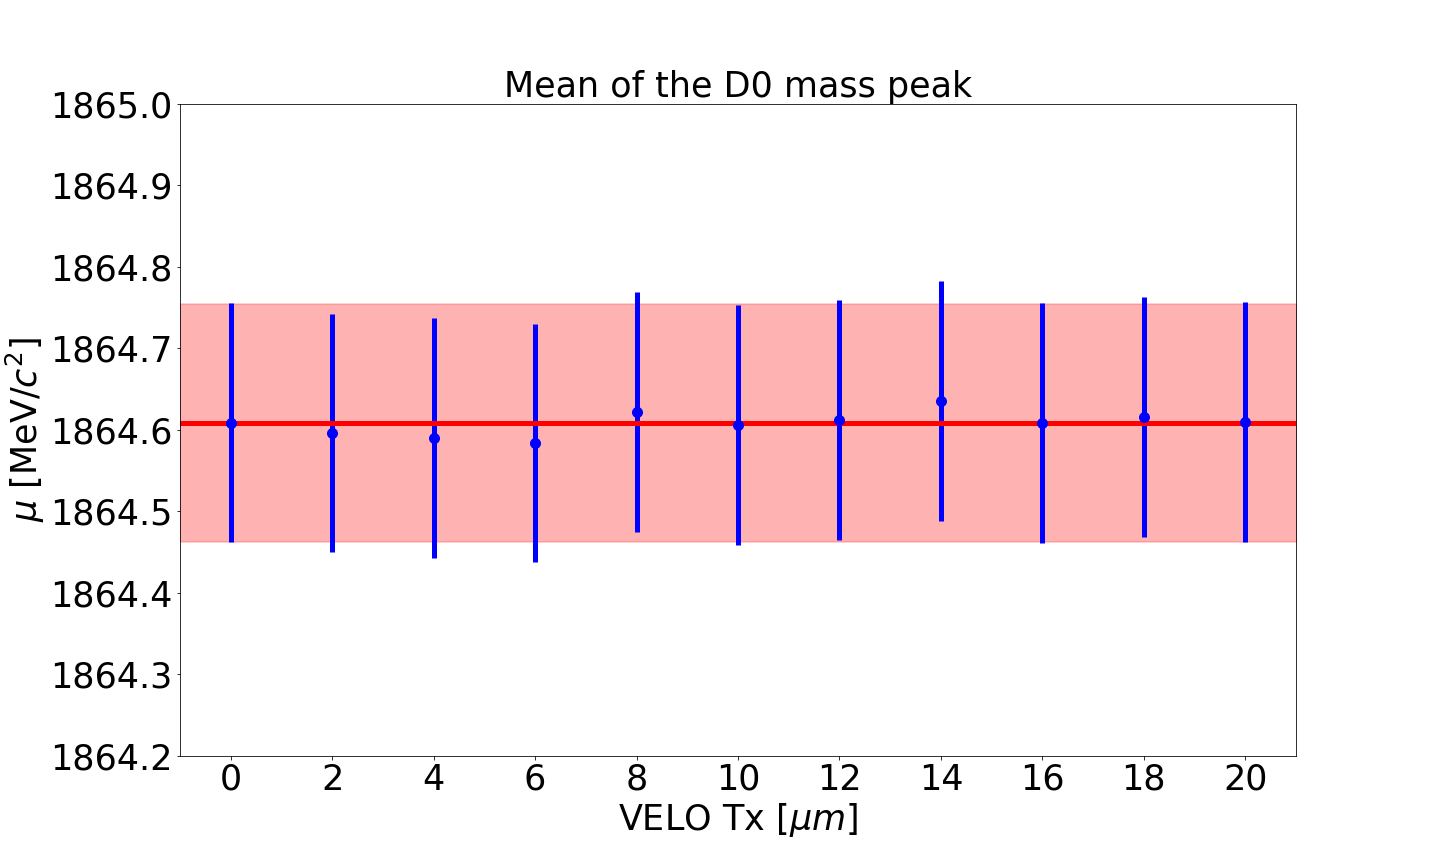
\includegraphics[width=0.5\textwidth]{reading_material/current_stuff/velo_drift_plots/plots/D0_massvalue_largeVPTx.png}
      \end{figure}
    \end{column}
  \end{columns}
\end{frame}

\begin{frame}\frametitle{VELO drift impact for SciFi alignment}
  \begin{columns}
    \begin{column}[c]{0.48\textwidth}
      \begin{figure}
        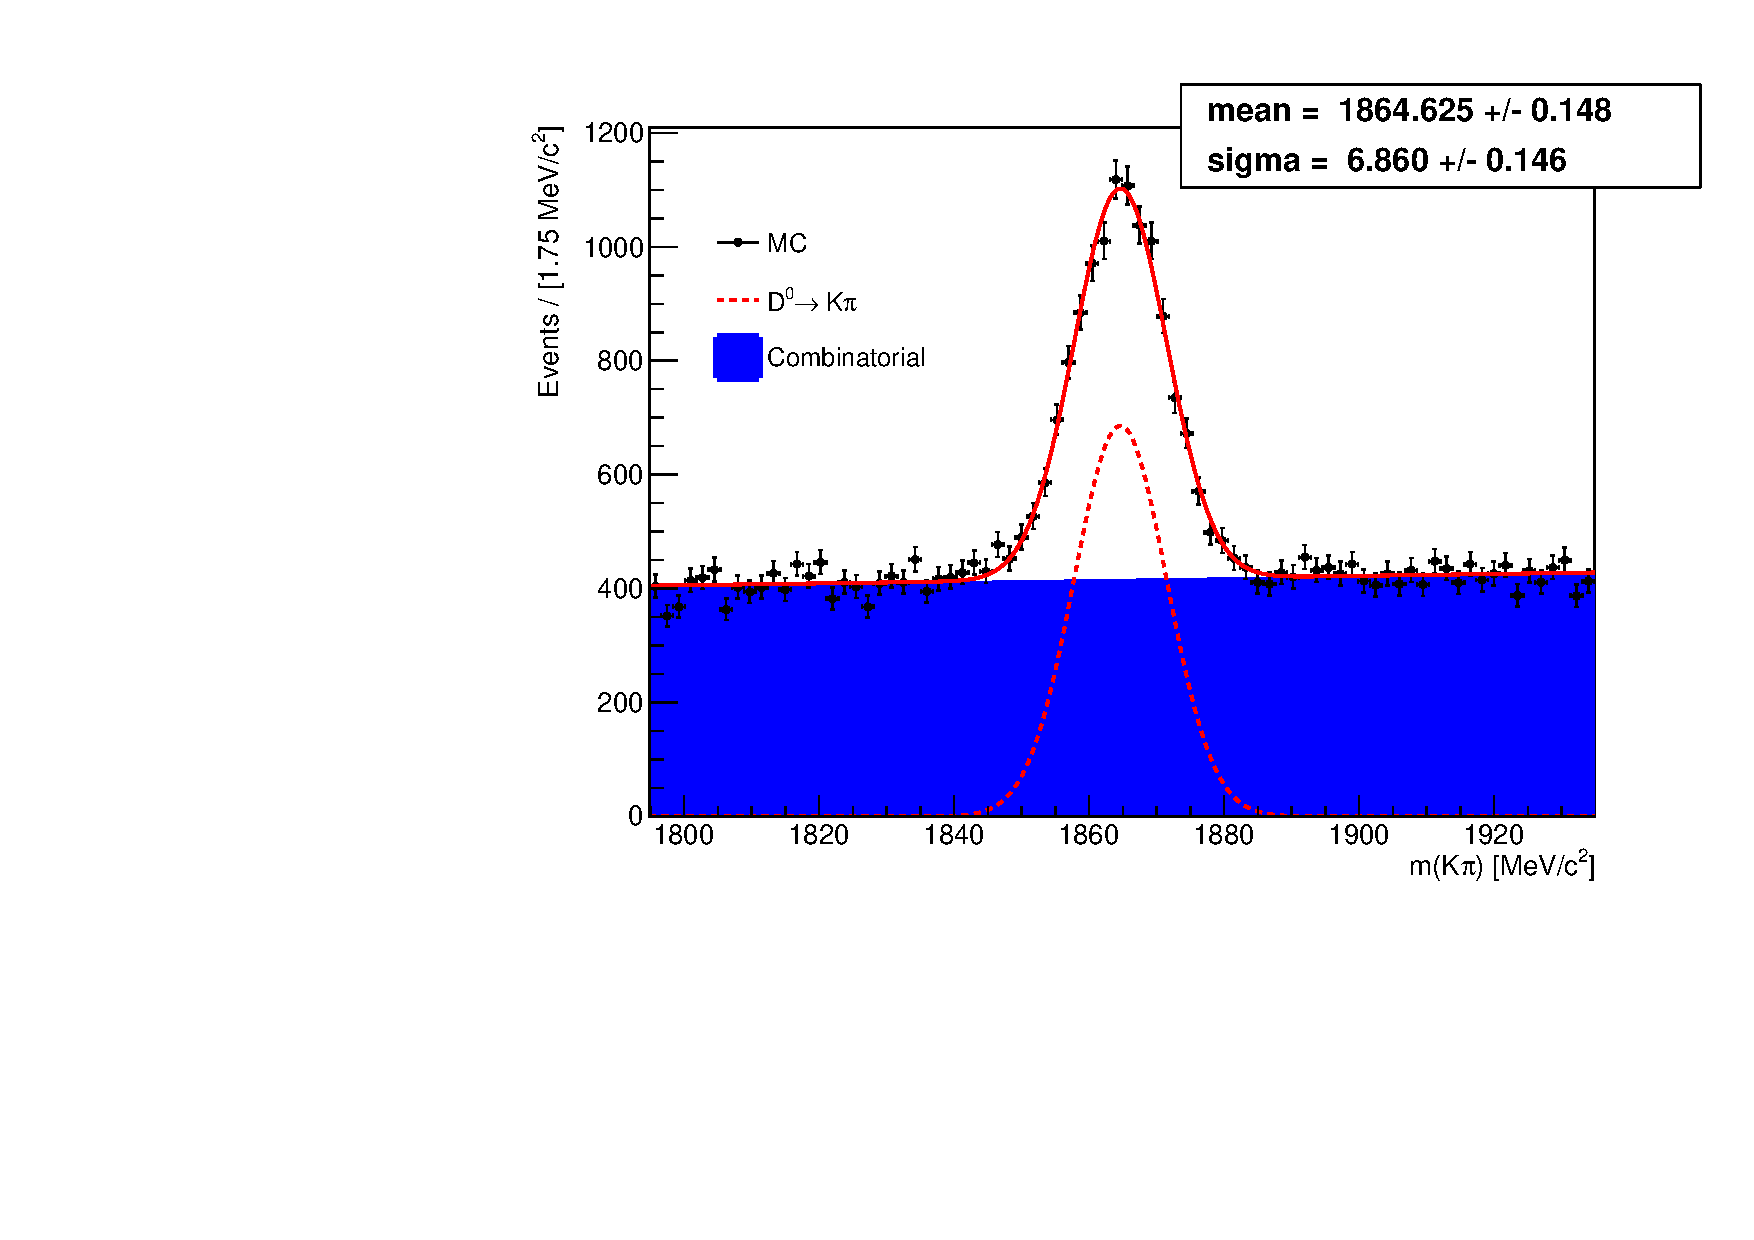
\includegraphics[width=0.8\textwidth]{reading_material/current_stuff/velo_drift_plots/plots/Fit_VpTx20Iter4.pdf}
      \end{figure}
    \end{column}
    \begin{column}[c]{0.48\textwidth}
      \begin{itemize}
        \item $\bullet$\, $\symbf{\symup{Ry}}$ shows no impact on SciFi alignment and mass distribution
        \item $\bullet$\, mass peak slightly affected for drifts below $20 \mu m$
        \item $\bullet$\, large movements impact on mass resolution visibly
        \item $\bullet$\, alignment with VELO drift also negatively impacts resolution slightly
      \end{itemize}
    \end{column}
  \end{columns}
\end{frame}

\begin{frame}\frametitle{SciFi alignment with 2022 data}
  \begin{columns}
    \begin{column}[c]{0.48\textwidth}
      \begin{figure}
        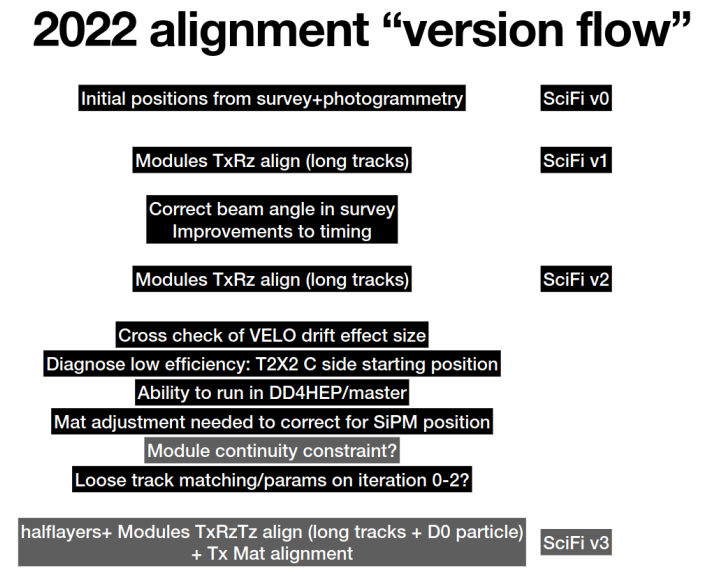
\includegraphics[width=0.9\textwidth]{plots/alignment_version_flow.png}
      \end{figure}
      from \href{https://indico.cern.ch/event/1275405/contributions/5372370/attachments/2636783/4562038/SciFiAlignUpdate_20230427.pdf}{Sophie's slides}
    \end{column}
    \begin{column}[c]{0.48\textwidth}
      \begin{itemize}
        \item $\bullet$\, half modules yield better performance than long modules
        \item $\bullet$\, why? becasue if starting conditions not quite correct, half modules can correct it better
        \item $\bullet$\, beam angle fix + better fine timing
        \item $\bullet$\, VELO z-drift studies (later in the talk)
        \item $\bullet$\, discovered low efficiency C-side \to improved starting conditions
        \item $\bullet$\, mats need to correct for SiPM positions
        \item $\bullet$\, loose track matching/params in first iterations yield performance boost
        \item $\bullet$\, Final v3: TxTzRz, halflayers + modules, long tracks to D0 particles + Tx mat alignment
      \end{itemize}
    \end{column}
  \end{columns}
\end{frame}

\begin{frame}\frametitle{SciFi Mats: from v9 to v10}
  \begin{columns}
    \begin{column}[c]{0.48\textwidth}
      \begin{figure}
        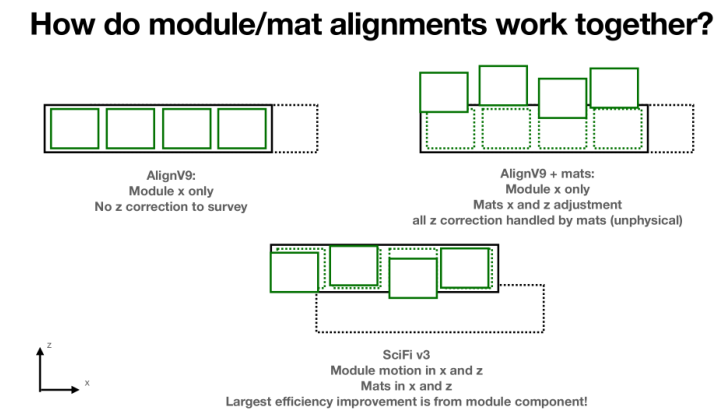
\includegraphics[width=0.9\textwidth]{plots/modules_and_mats.png}
      \end{figure}
    \end{column}
    \begin{column}[c]{0.48\textwidth}
      \begin{itemize}
        \item $\bullet$\, v9 featured no z correction in survey and shifting of whole module in x
        \item $\bullet$\, v9 + mats: SiPMs being aligned and not glued mats
        \item $\bullet$\, \to still unphysical movement out of the module
        \item $\bullet$\, v10: modules movement in x and z allows for physical 'mat movement'
        \item $\bullet$\, yield: largest efficiency improvement from module alignment but mats needed
      \end{itemize}
    \end{column}
  \end{columns}
\end{frame}

\begin{frame}\frametitle{Mat alignment}
  \begin{columns}
    \begin{column}[c]{0.48\textwidth}
      from \href{https://indico.cern.ch/event/1275394/contributions/5359493/attachments/2628409/4549668/SciFi_mat_alignment.pdf}{Zehua's slides}
      \begin{figure}
        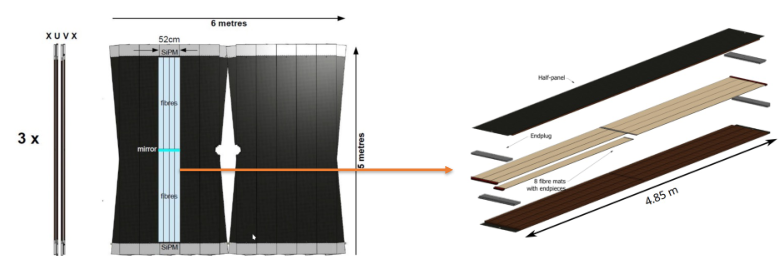
\includegraphics[width=0.9\textwidth]{plots/scifi_mats.png}
      \end{figure}
    \end{column}
    \begin{column}[c]{0.48\textwidth}
      \begin{itemize}
        \item $\bullet$\, real mats glued together with fine tolerance
        \item $\bullet$\, but preliminary mat alignment sees movement up to 1.5mm
        \item $\bullet$\, Mat alignment: moving mats in software to match best hit position in tracking
        \begin{itemize}
          \item $\bullet$\, depends on module alignment quality
          \item $\bullet$\, depends on relative position of glued SiPM readout relativ to mats
        \end{itemize}
      \end{itemize}
    \end{column}
  \end{columns}
\end{frame}

\begin{frame}\frametitle{Summary}
  \begin{columns}
    \begin{column}[c]{0.48\textwidth}

    \end{column}
    \begin{column}[c]{0.48\textwidth}
      \to Goal:
      \begin{itemize}
        \item $\bullet$\, correct for hit positions in readout without moving mat material in simulation
        \item $\bullet$\, understand rotations in survey positions that may produce z movement in reco
        \item $\bullet$\, understand true variations in SiPM positions
      \end{itemize}
    \end{column}
  \end{columns}
\end{frame}

% \begin{frame}\frametitle{}
%   \begin{columns}
%     \begin{column}[c]{0.48\textwidth}
%
%     \end{column}
%     \begin{column}[c]{0.48\textwidth}
%
%     \end{column}
%   \end{columns}
% \end{frame}

\begin{frame}\frametitle{Monitoring}

\end{frame}

\begin{frame}\frametitle{Cluster bias}

\end{frame}

\end{document}
